\documentclass{article}

% 1 inch margins
\usepackage[margin=1in]{geometry}

% Link
\usepackage{hyperref}

% Prevent paragraph indentation
\usepackage{parskip}

% Image
\usepackage{graphicx}

% Page header
\usepackage{fancyhdr}
\pagestyle{fancy}
\lhead{Jai Wargacki}
\rhead{CSCI-711-01 Global Illumination\\ Midterm Update}

\begin{document}
% Title -- A short (ideally) but catchy name for your project; essentially, a summary of what you're doing in a few words.
\textbf{Title:} Dash Cam Path Visualization

% Name(s) -- Your name (if you are working alone), or a list of the names of the members of the team (if working as a team) with an indication of who is the team leader.
\textbf{Name:} Jai Wargacki

% Class name and number -- CSCI-711, Global Illumination.
\textbf{Class:} CSCI-711, Global Illumination

% Project web site URL -- This is where you'll post all your project-related material (including your proposal).
\textbf{Project URL:} \url{https://cs.rit.edu/~jpw5681/cs711/Website/}

% Summary of the project -- A description of the 3D scene that is to be constructed, the aspect of the rendering pipeline that will be emphasized, and the means by which you plan on doing so.
\textbf{Summary:} The goal of this project is to create a visualization of a recorded dash cam path on a 3D map.
Additionally, when the user mouses over the path, a thumbnail of the video at that point will be displayed for the user to view.
This project will emphasize interactivity. The user is able to move the camera around the scene to view the path from different angles
as well as hover the mouse over the path to view the video at that point. This project will be accomplished by adding additional 3D elements to 
webGL elements provided by the Google Maps API. It is currently unclear what will be needed additionally to plot a smooth path on the map, and
display the video thumbnails over the route.

\textbf{Progress:} So far I have a webGL application running that is able to display a 3D map using the Google Maps API. 
I am able to draw 3D object onto the map and move the camera around the scene (through user control or programmatically).
My application is able to load path coordinates from a file and create what I am calling a "path" object. I am 
in the process of drawing the path onto the map.

% Screenshot
\begin{figure}[h]
\centering
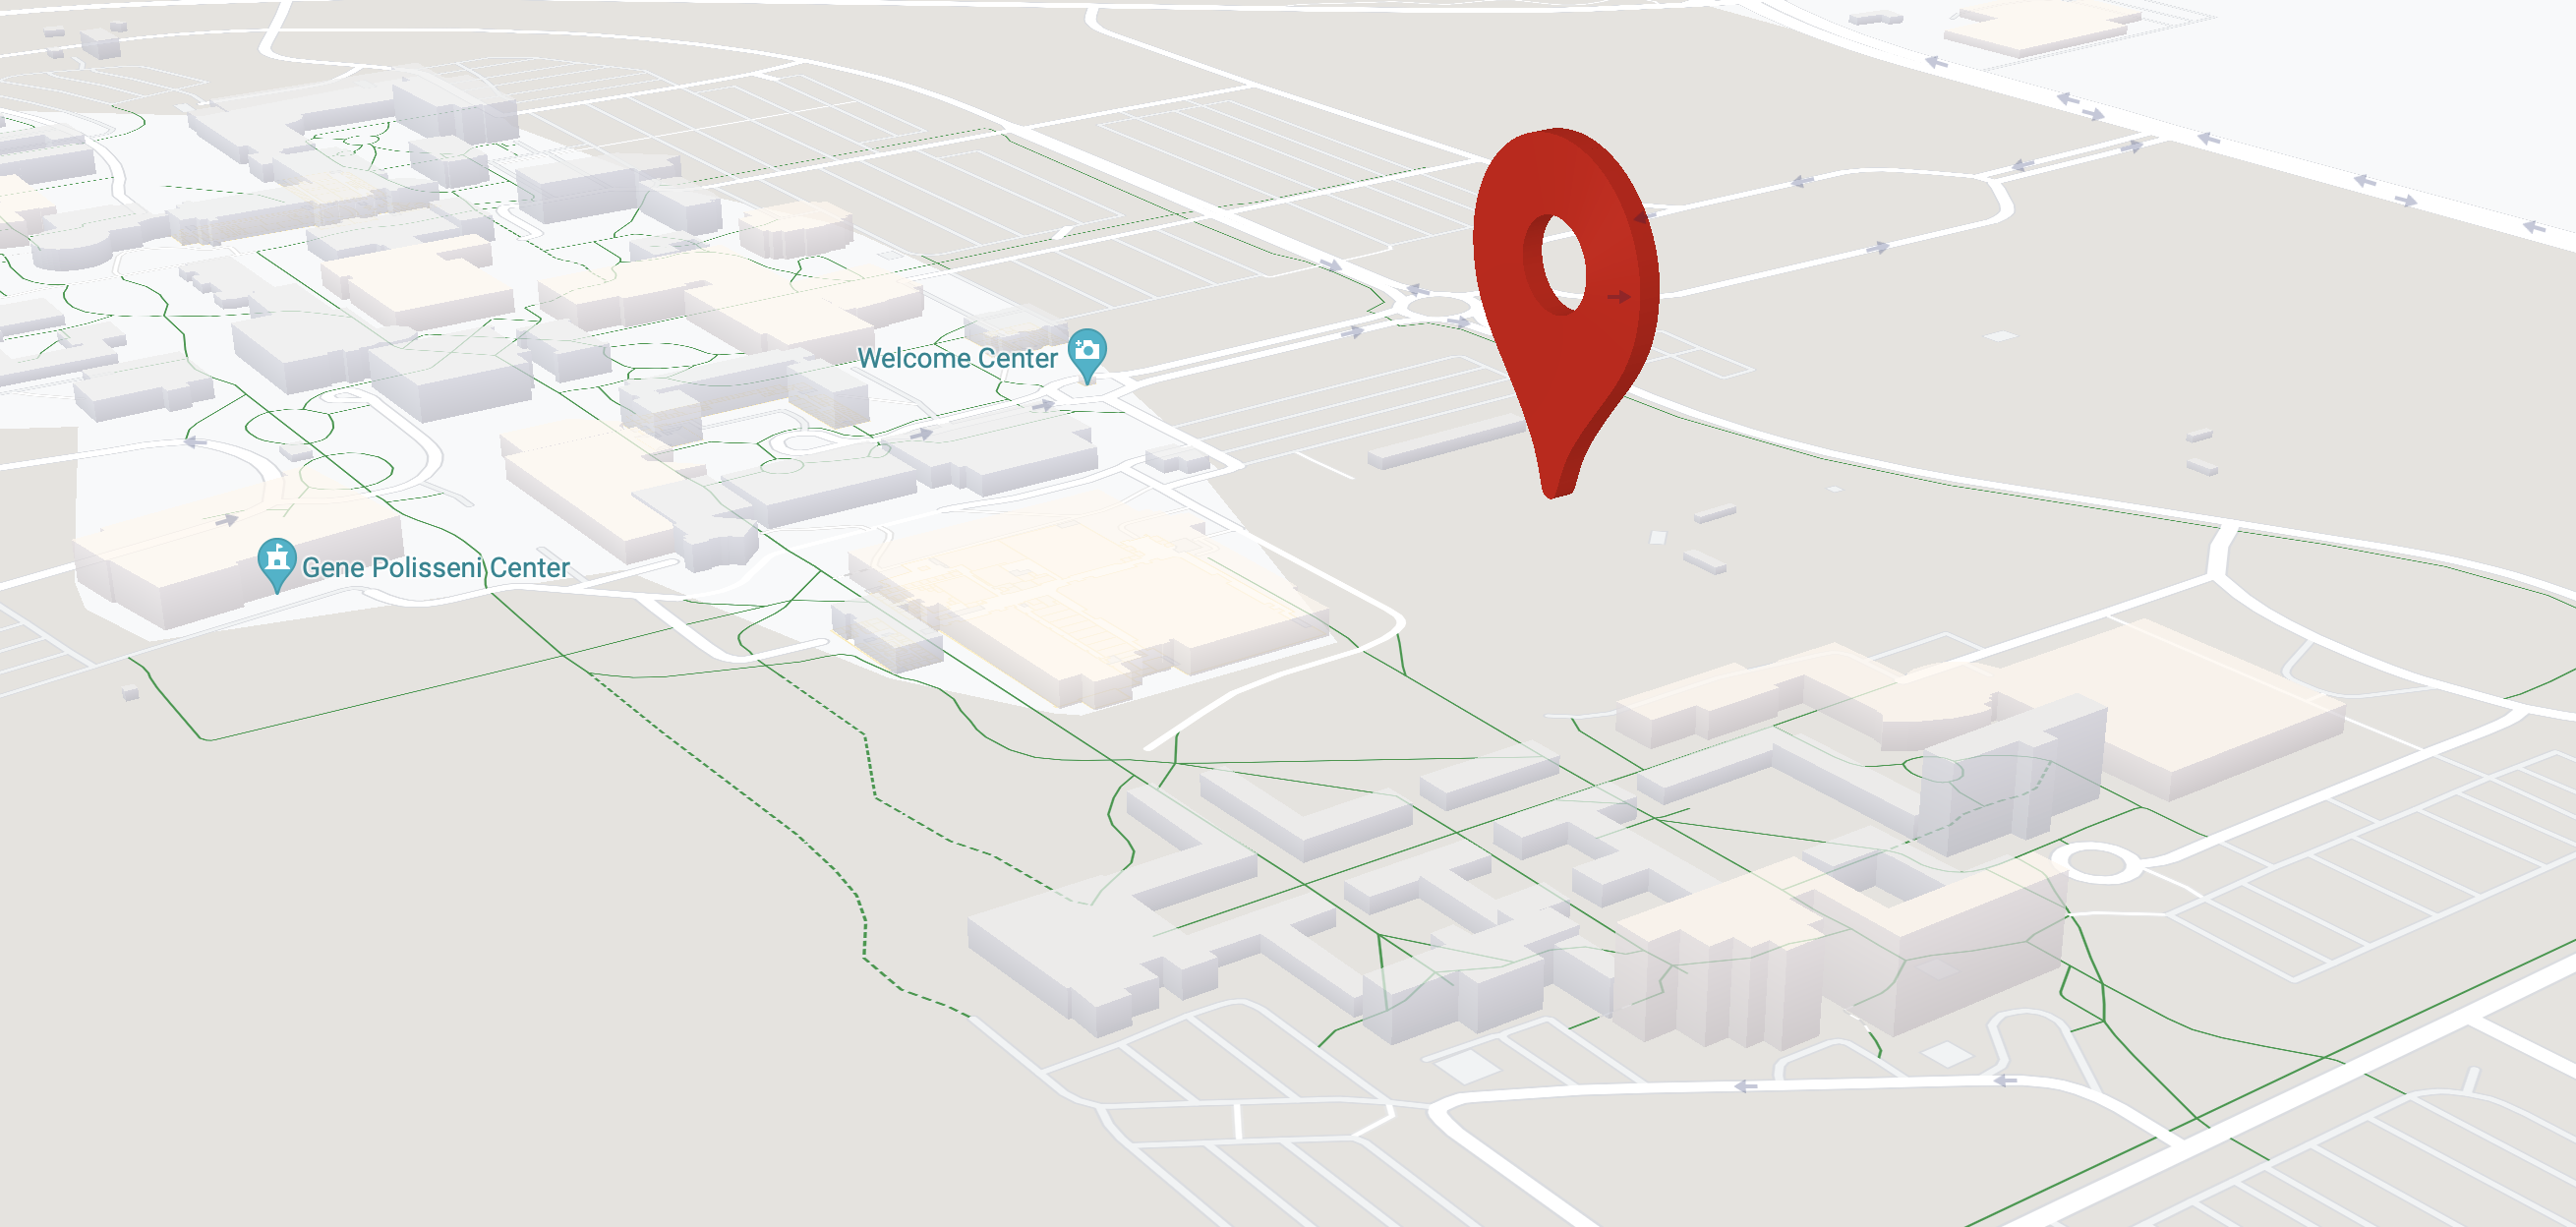
\includegraphics[width=0.5\textwidth]{screenshot.png}
\caption{3D map with a 3D object drawn on it.}
\end{figure}

\textbf{Remaining Tasks:} The remaining parts of my project are to draw the path onto the map, display the video thumbnails over the path,
and clean up the user interface. I want to accomplish the MVP of this project before I start worrying about smaller details like the 
exact styling of the map. As I complete these tasks I will also determine how I plan on integrating this project with 
my capstone project.

\textbf{Assessment of Progress:} I am on track to complete the project in my originally planned time frame. So far I have been able to
complete the tasks I have set out for myself on schedule with my original plan.
\end{document}